The ClockAlarm project is an application allowing the user to manage alarms which will alert him at specified times. The user can create new alarms and assign them to categories in order to stay organised. The project is thought to replace in the long run an existing application named \gls{kalarm}.

\begin{figure}[h]
\centering
\caption{\gls{kalarm} main window on KDE}
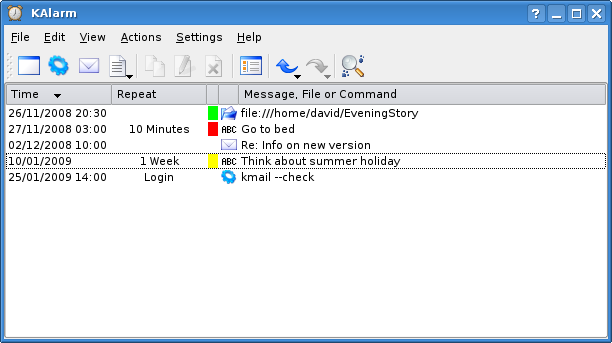
\includegraphics[width=0.7\textwidth]{kalarm.png}
\end{figure}